

In Figures \ref{fig:SA_BUNNY}, \ref{fig:SA_FANDISK} and \ref{fig:SA_HORSE} we compare the Plane-Tree with the state-of-the-art transform methods by Bayazit et al. \cite{Bayazit103DMesh}, Khodakovsky et al. \cite{Khodakovsky00Progressive} and the SOT \cite{Lincoln13Hons}. \\

Experiment results comparing the Plane-Tree compression system proposed in this work with the transform-based method by Khodakovsky et al. and SOT are shown in figure \ref{fig:SA_BUNNY}. This Rate-Distortion graph shows that the Plane-Tree has similar performance with the method by Khodakovsky et al. At low bit-rates the Plane-Tree is highly competitive the with performance matching Khodakovsky's. The SOT method outperforms both of these data structures at lower bit-rates. \\

Figure \ref{fig:SA_FANDISK} shows comparisons between the Plane-Tree as well as methods by Khodakovsky et al., Bayazit et al. and the SOT. Here, both the Plane-Tree and the method by Khodakovsky et al. perform similarly as in the bunny model experiment (Figure \ref{fig:SA_BUNNY}). The Plane-Tree stays competitive with that state-of-the-art method, and improves upon the compression performance in comparison to the spectral compression method by Bayazit et al. and the SOT. It can be seen that at low to mid bit-rates, the Plane-Tree method compressed the Fandisk model at a higher level of quality for a given bit-rate. \\

The Plane-Tree was also compared with Bayazit et al. and the SOT using another model, the horse model. Figure \ref{fig:SA_HORSE} shows the result of this experiment. The Plane-Tree method outperforms the transform based method of Bayazit et al. and the SOT whilst decreasing coding complexity compared to the complicated transform method. Overall, in this experiment, the proposed Plane-Tree method remains competitive at higher bitrates, and it outperforms the method by Bayazit et al. at lower bitrates. \\

Finally, the Plane-Tree is compared with the state-of-the-art low-bitrate compression system FOLProM presented by Peng et al. \cite{Peng10Feature} (as well as the SOT). Unlike the other experiments, the mean-error metric is used in this comparison, as the results presented by Peng et al. used this metric. It can be seen that at low bit-rates (below 2 bits per vertex), the Plane-Tree method outperforms this state-of-the-art low-bitrate compression system. Moreover, the Plane-Tree easily outperforms the SOT. \\


In conclusion, these experiments show that the Plane-Tree is extremely competitive with the state-of-the-art compression systems at high bit-rates. At lower bit-rates it improves upon the results by these methods. In three out of the four experiments, the Plane-Tree outperformed the SOT. The Plane-Tree is also powerful in that it may be used to compress 3D volumetric data as well as point-cloud and mesh data. This makes it an interesting candidate for 3D reconstruction compression no matter the format output by a given 3D reconstruction method. \\

\begin{figure}[!htb] 
        \centering
        \begin{subfigure}[b]{1.8in}
                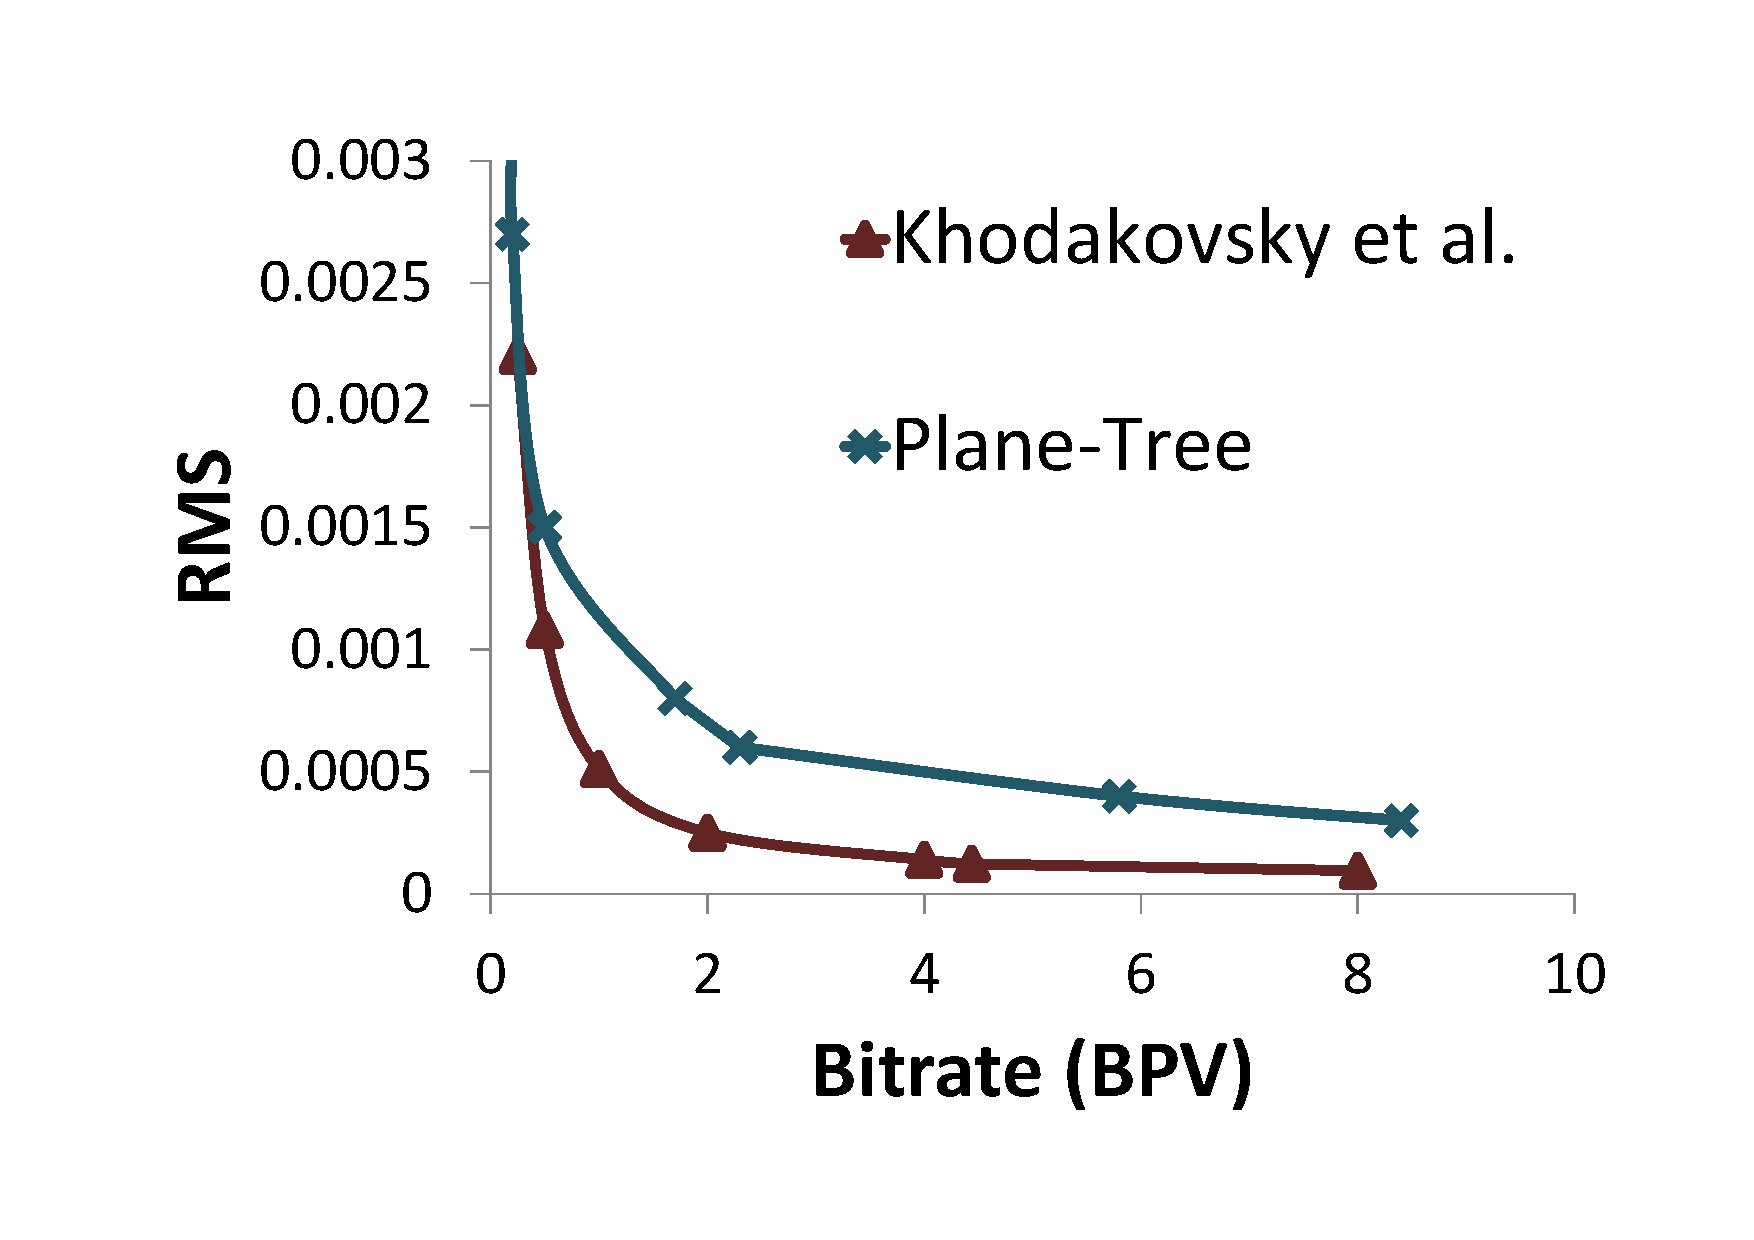
\includegraphics[width=1.8in]{images/results/compression/bunnysota}
                \caption{Bunny Model}
                \label{fig:SA_BUNNY}
        \end{subfigure}%
        \begin{subfigure}[b]{1.8in}
                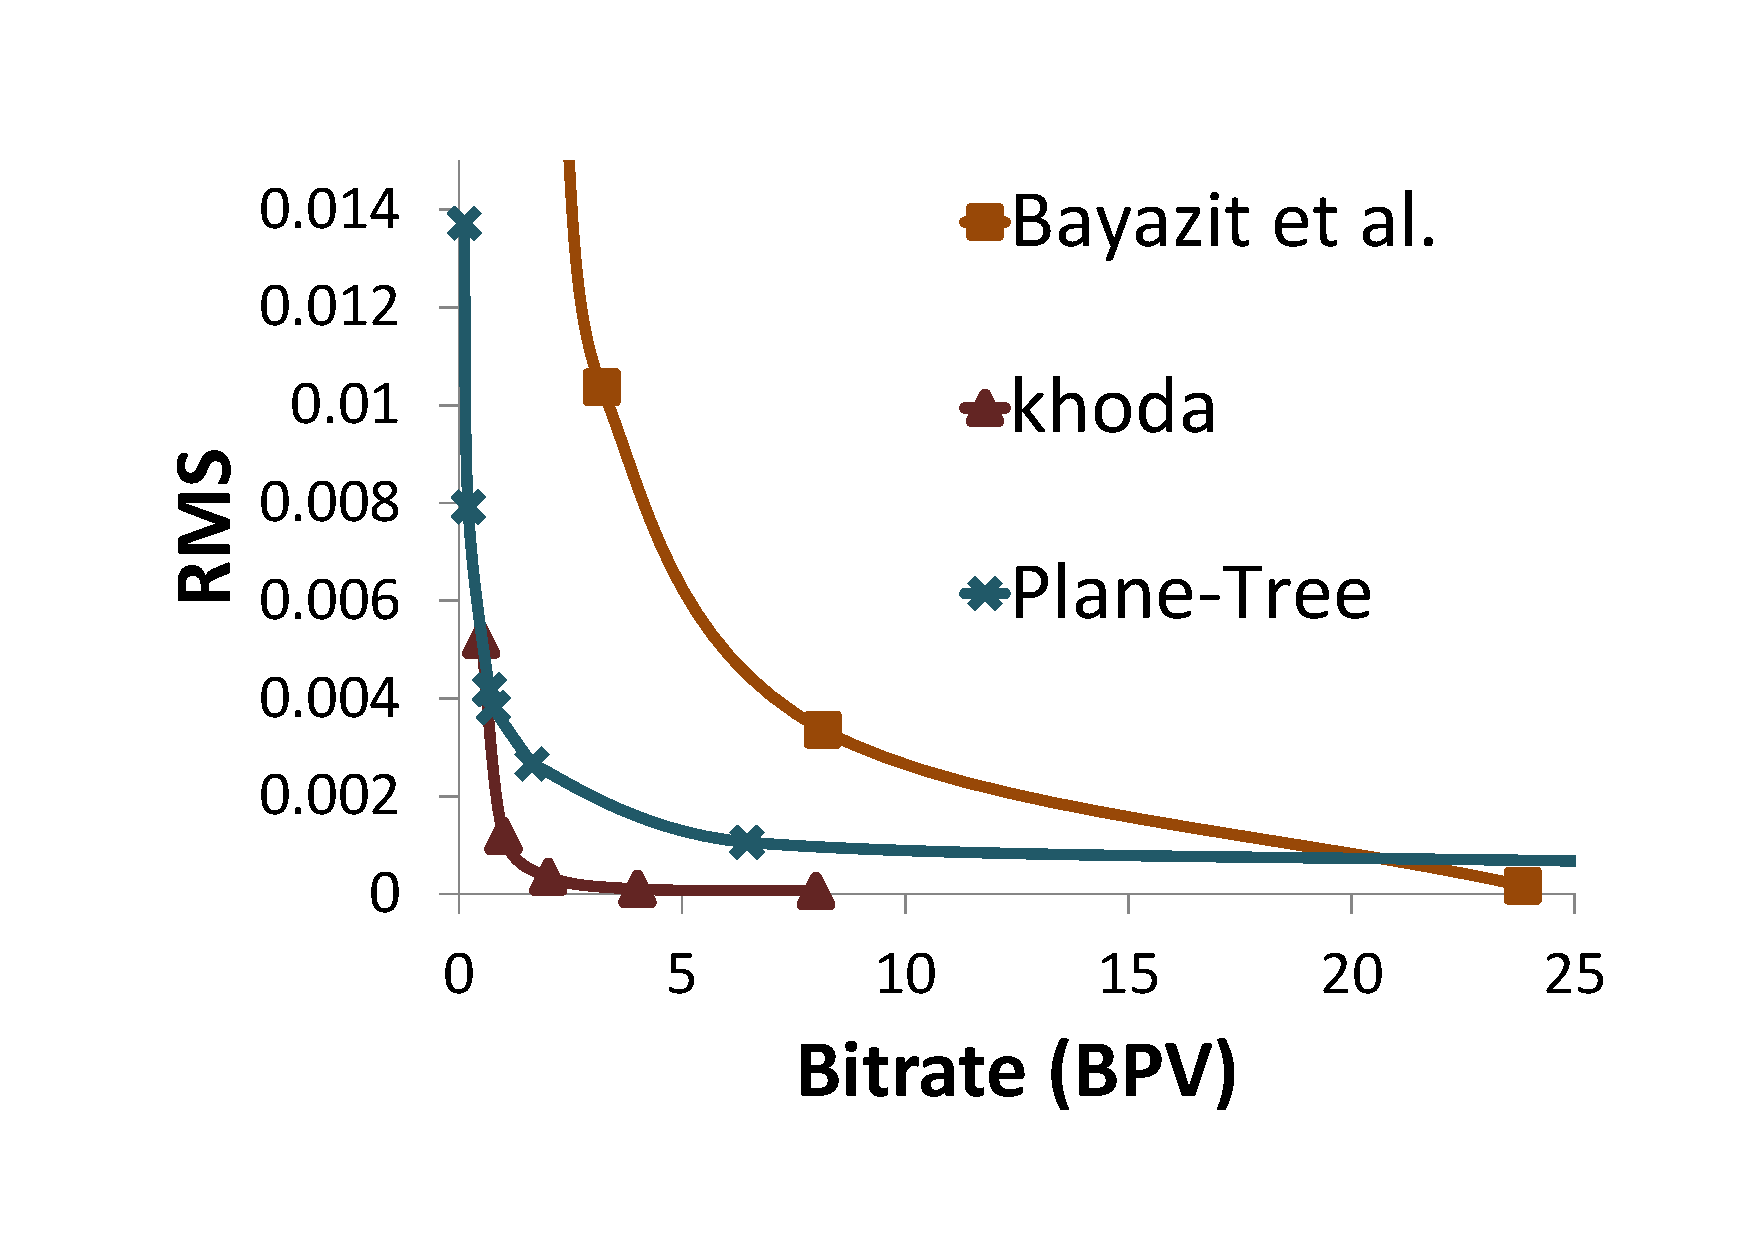
\includegraphics[width=1.8in]{images/results/compression/fandisksota}
                \caption{Fandisk Model}
                \label{fig:SA_FANDISK}
        \end{subfigure}
        
        \begin{subfigure}[b]{1.8in}
                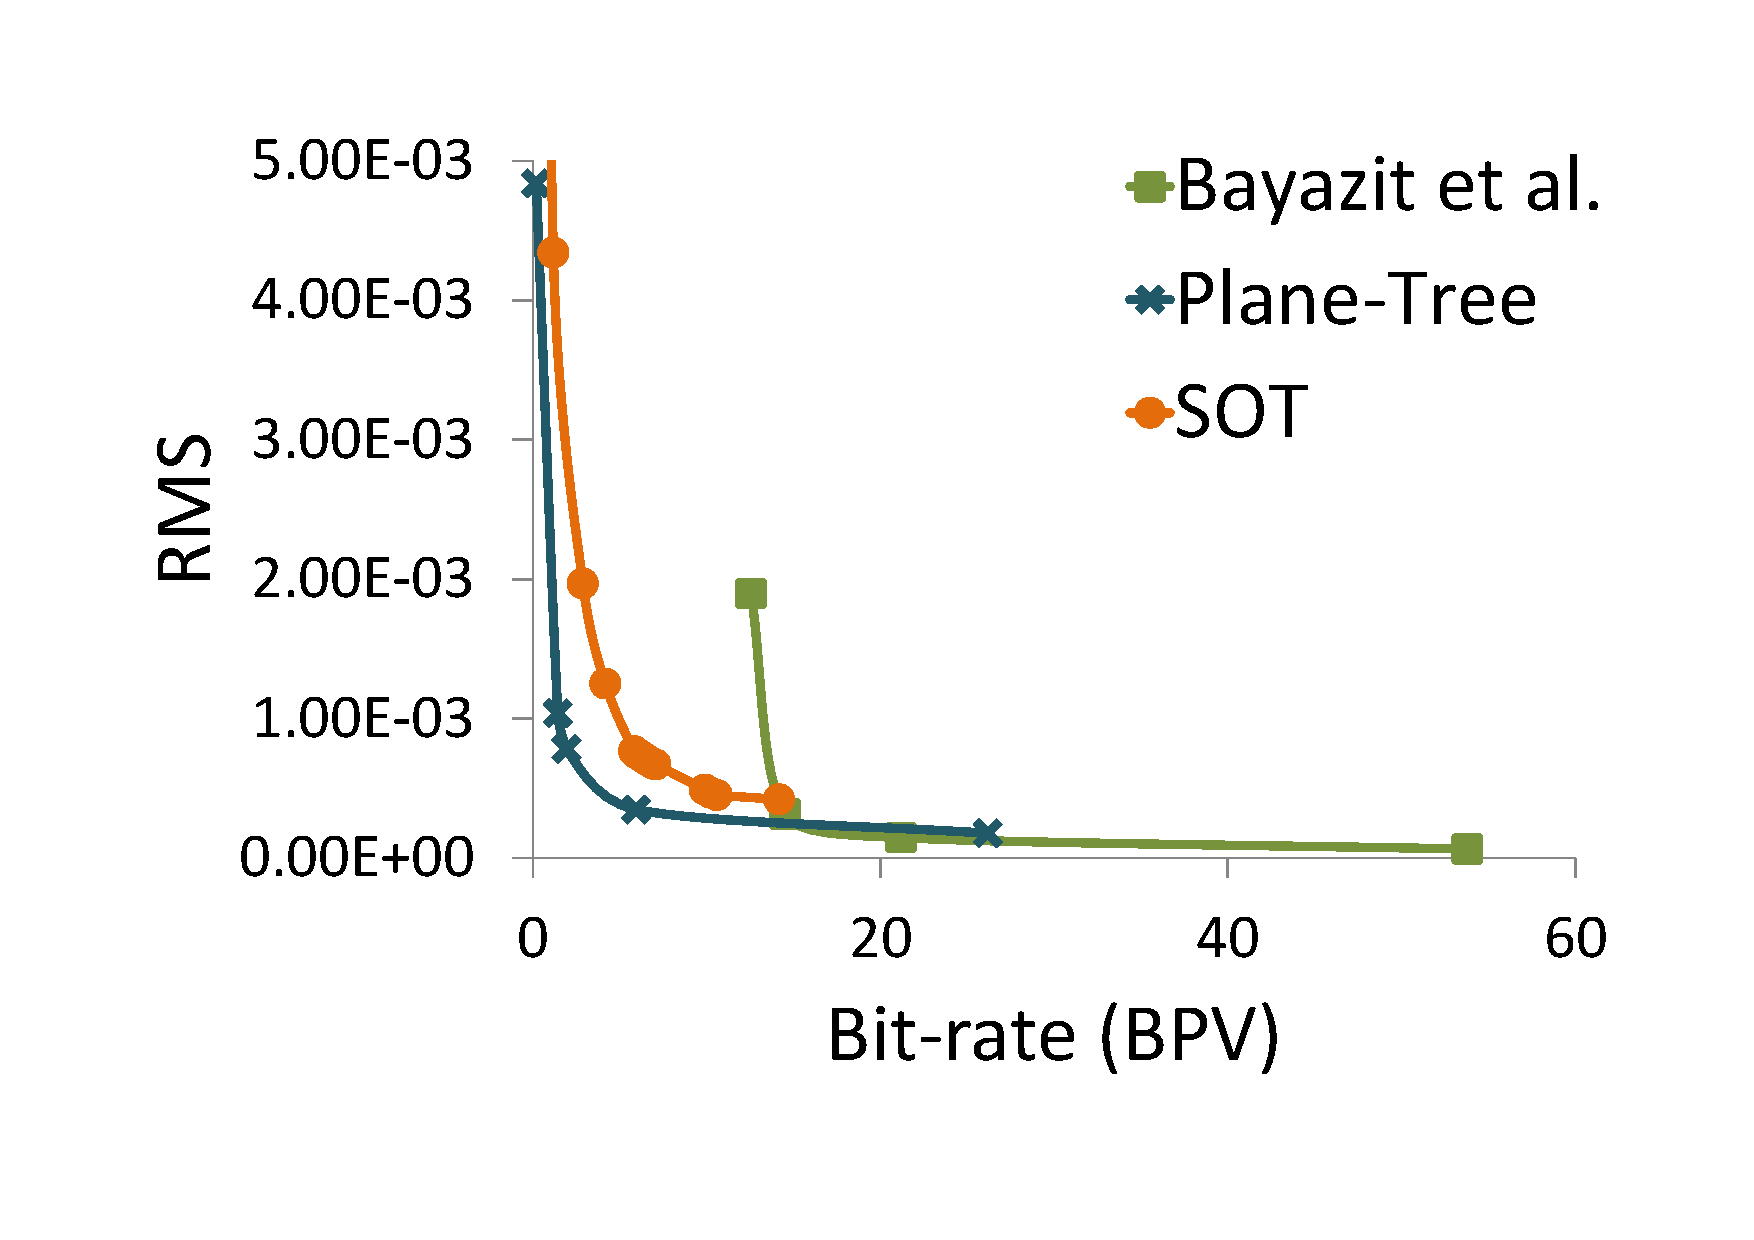
\includegraphics[width=1.8in]{images/results/compression/horsesota}
                \caption{Horse Model}
                \label{fig:SA_HORSE}
        \end{subfigure}%
        \begin{subfigure}[b]{1.8in}
                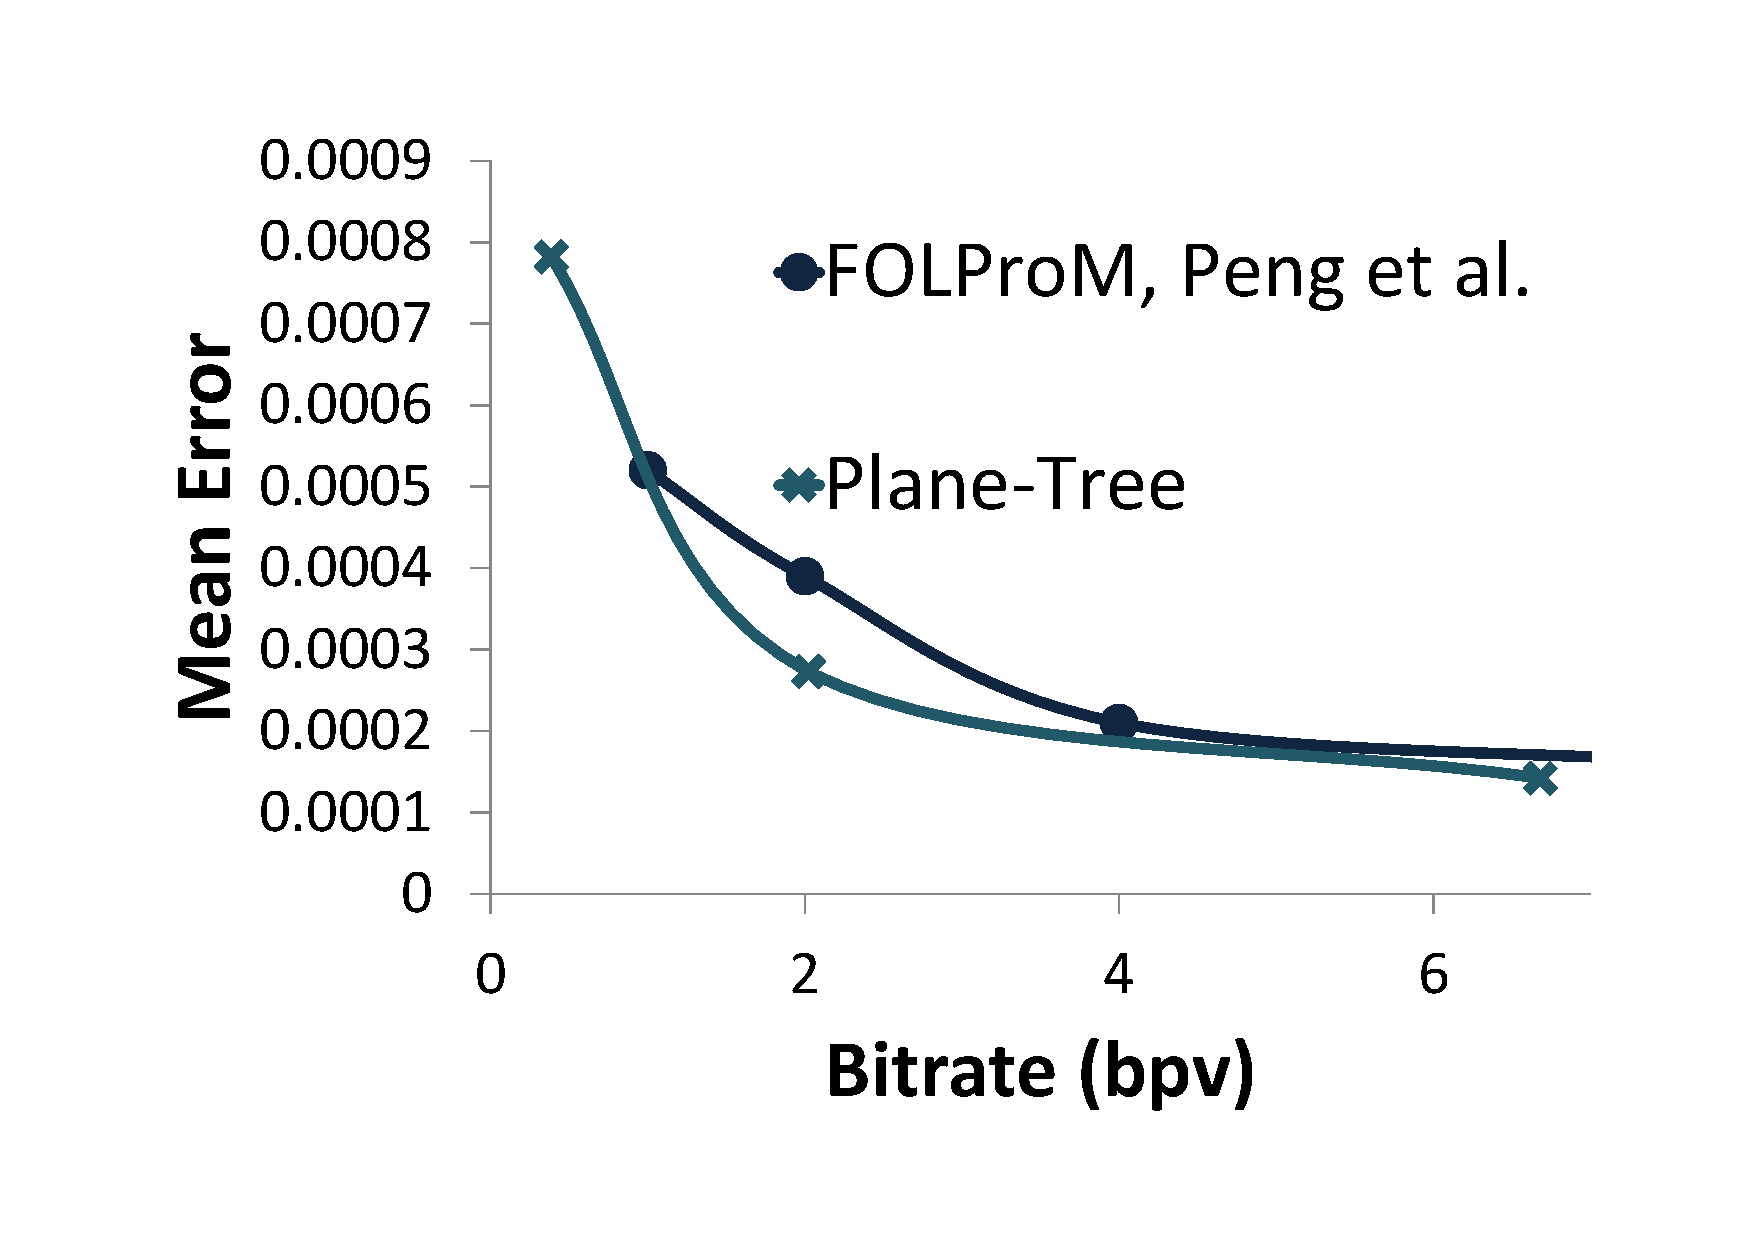
\includegraphics[width=1.8in]{images/results/compression/rabbitsota}
                \caption{Rabbit Model}
                \label{fig:SA_RABBIT}
        \end{subfigure}
       \caption{Rate-Distortion graphs comparing the Plane-Tree to different state of the art codecs.}
       \label{fig:SOTAEXPS}
\end{figure}